\documentclass[12pt,a4paper]{article}

% ─── Packages ─────────────────────────────────────────────
\usepackage[utf8]{inputenc}
\usepackage[T1]{fontenc}
\usepackage{lmodern}
\usepackage{amssymb}
\usepackage[margin=2.5cm]{geometry}
\usepackage{graphicx}
\usepackage{xcolor}
\usepackage{tikz}
\usetikzlibrary{arrows.meta, positioning, shapes.geometric, fit, calc}
\usepackage{booktabs}
\usepackage{enumitem}
\usepackage{hyperref}
\usepackage{fancyhdr}
\usepackage{tcolorbox}
\usepackage{multirow}
\usepackage{longtable}
\usepackage{array}

\tcbuselibrary{skins, breakable}

% ─── Colors ───────────────────────────────────────────────
\definecolor{personA}{HTML}{4A90D9}   % Blue
\definecolor{personB}{HTML}{E67E22}   % Orange
\definecolor{personC}{HTML}{27AE60}   % Green
\definecolor{personD}{HTML}{8E44AD}   % Purple
\definecolor{depArrow}{HTML}{C0392B}  % Red for dependency arrows
\definecolor{sectionbg}{HTML}{ECF0F1}

% ─── Header / Footer ─────────────────────────────────────
\pagestyle{fancy}
\fancyhf{}
\lhead{\textbf{CMP3060 -- Phase 1 Task Division}}
\rhead{\today}
\cfoot{\thepage}

% ─── Title ────────────────────────────────────────────────
\title{%
  \vspace{-1cm}
  \textbf{CMP3060 Computer Graphics Project}\\[6pt]
  \Large Phase 1 --- Requirements Analysis \& Task Division
}
\author{Team Plan Document}
\date{\today}

\begin{document}
\maketitle
\thispagestyle{fancy}

% ══════════════════════════════════════════════════════════
\section{Phase 1 Requirements Overview}
% ══════════════════════════════════════════════════════════

Phase 1 consists of \textbf{11 requirements} that progressively build the OpenGL rendering engine. Each requirement involves completing \texttt{TODO} items in specific source files and shaders.

\begin{center}
\renewcommand{\arraystretch}{1.3}
\begin{tabular}{c l p{7.5cm}}
\toprule
\textbf{Req.} & \textbf{Name} & \textbf{Key Files} \\
\midrule
R1 & Shader Program &
  \texttt{shader.hpp/cpp}, \texttt{triangle.vert},
  \texttt{color-mixer.frag}, \texttt{checkerboard.frag} \\
R2 & Mesh &
  \texttt{mesh.hpp} \\
R3 & Transform &
  \texttt{transform.cpp}, \texttt{transform-test.vert} \\
R4 & Pipeline State &
  \texttt{pipeline-state.hpp} \\
R5 & Texture &
  \texttt{texture2d.hpp}, \texttt{texture-utils.cpp},
  \texttt{texture-test.frag} \\
R6 & Sampler &
  \texttt{sampler.hpp/cpp} \\
R7 & Material &
  \texttt{material.cpp}, \texttt{tinted.frag},
  \texttt{textured.frag} \\
R8 & Entities \& Components &
  \texttt{entity.hpp/cpp}, \texttt{world.hpp/cpp},
  \texttt{camera.cpp}, \texttt{mesh-renderer.cpp},
  \texttt{component-deserializer.hpp},
  \texttt{entity-test-state.hpp} \\
R9 & Forward Renderer &
  \texttt{forward-renderer.hpp} \\
R10 & Sky Rendering &
  \texttt{forward-renderer.hpp} (additional TODOs) \\
R11 & Postprocessing &
  \texttt{forward-renderer.hpp}, \texttt{texture-utils.cpp},
  \texttt{vignette.frag}, \texttt{chromatic-aberration.frag} \\
\bottomrule
\end{tabular}
\end{center}

% ══════════════════════════════════════════════════════════
\section{Dependency Analysis}
% ══════════════════════════════════════════════════════════

The following diagram shows the dependency graph. An arrow $A \to B$ means ``\emph{B depends on A}'' (i.e.\ A must be completed before B).

\begin{center}
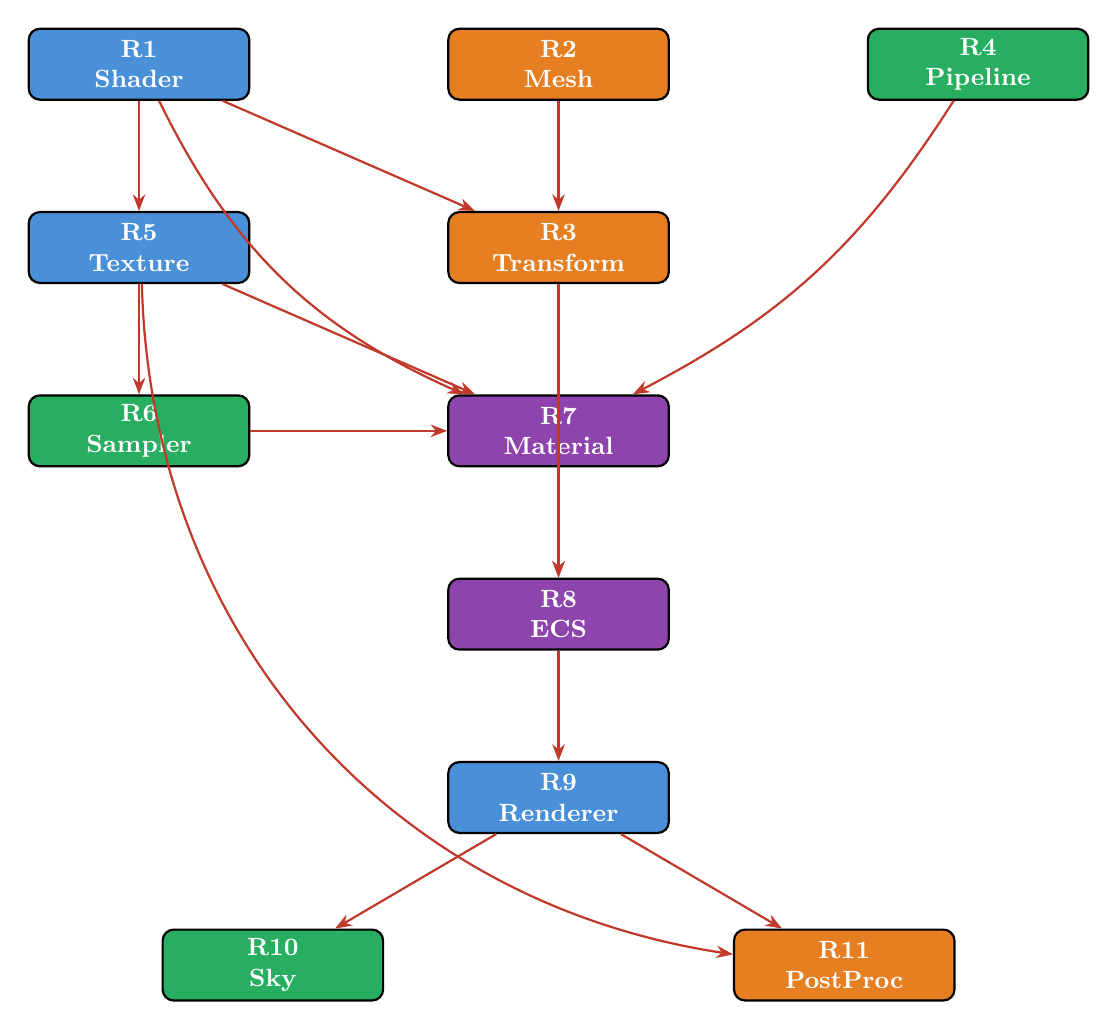
\begin{tikzpicture}[
    node distance=1.4cm and 2.0cm,
    req/.style={
      rectangle, rounded corners=4pt, draw, thick,
      minimum width=2.8cm, minimum height=0.9cm,
      font=\small\bfseries, text=white, align=center
    },
    dep/.style={-{Stealth[length=6pt]}, thick, depArrow},
  ]

  %% ── Layer 0 (Independent / foundational) ──
  \node[req, fill=personA]                       (R1) {R1\\Shader};
  \node[req, fill=personB, right=2.5cm of R1]    (R2) {R2\\Mesh};
  \node[req, fill=personC, right=2.5cm of R2]    (R4) {R4\\Pipeline};

  %% ── Layer 1 ──
  \node[req, fill=personA, below=of R1]           (R5) {R5\\Texture};
  \node[req, fill=personB, below=of R2]           (R3) {R3\\Transform};

  %% ── Layer 2 ──
  \node[req, fill=personC, below=of R5]           (R6) {R6\\Sampler};

  %% ── Layer 3 ──
  \node[req, fill=personD, below=of R3]           (R7) {R7\\Material};

  %% ── Layer 4 ──
  \node[req, fill=personD, below=of R7]           (R8) {R8\\ECS};

  %% ── Layer 5 ──
  \node[req, fill=personA, below=of R8]           (R9) {R9\\Renderer};

  %% ── Layer 6 ──
  \node[req, fill=personC, below left=1.2cm and 0.8cm of R9]  (R10) {R10\\Sky};
  \node[req, fill=personB, below right=1.2cm and 0.8cm of R9] (R11) {R11\\PostProc};

  %% ── Dependency arrows ──
  \draw[dep] (R1) -- (R5);
  \draw[dep] (R1) -- (R3);
  \draw[dep] (R2) -- (R3);
  \draw[dep] (R5) -- (R6);
  \draw[dep] (R1) to[bend right=20] (R7);
  \draw[dep] (R4) to[bend left=15] (R7);
  \draw[dep] (R5) -- (R7);
  \draw[dep] (R6) -- (R7);
  \draw[dep] (R7) -- (R8);
  \draw[dep] (R3) -- (R8);
  \draw[dep] (R8) -- (R9);
  \draw[dep] (R9) -- (R10);
  \draw[dep] (R9) -- (R11);
  \draw[dep] (R5) to[bend right=40] (R11);

\end{tikzpicture}
\end{center}

\subsection{Dependency Table}

\begin{center}
\renewcommand{\arraystretch}{1.25}
\begin{tabular}{c l l l}
\toprule
\textbf{Req.} & \textbf{Name} & \textbf{Depends On} & \textbf{Needed By} \\
\midrule
R1  & Shader         & ---                 & R3, R5, R7 \\
R2  & Mesh           & ---                 & R3 \\
R3  & Transform      & R1, R2              & R8 \\
R4  & Pipeline State & ---                 & R7 \\
R5  & Texture        & R1                  & R6, R7, R11 \\
R6  & Sampler        & R5                  & R7 \\
R7  & Material       & R1, R4, R5, R6      & R8 \\
R8  & ECS            & R3, R7              & R9 \\
R9  & Forward Renderer & R8                & R10, R11 \\
R10 & Sky Rendering  & R9                  & --- \\
R11 & Postprocessing & R9, R5              & --- \\
\bottomrule
\end{tabular}
\end{center}

% ══════════════════════════════════════════════════════════
\section{Task Division (4 Team Members)}
% ══════════════════════════════════════════════════════════

Based on the dependency analysis, the work is divided to:
\begin{itemize}[nosep]
  \item Maximize \textbf{parallelism} --- independent requirements start simultaneously.
  \item Balance \textbf{workload} --- measured by number of files and complexity.
  \item Minimize \textbf{blocking} --- tasks that block others are assigned to start first.
\end{itemize}

% ─── Color legend ─────────────────────────────────────────
\begin{center}

\begin{tikzpicture}
  \node[fill=personA, text=white, rounded corners=3pt, minimum width=2.5cm, minimum height=0.6cm, font=\bfseries] at (0,0) {Person A};
  \node[fill=personB, text=white, rounded corners=3pt, minimum width=2.5cm, minimum height=0.6cm, font=\bfseries] at (3.5,0) {Person B};
  \node[fill=personC, text=white, rounded corners=3pt, minimum width=2.5cm, minimum height=0.6cm, font=\bfseries] at (7,0) {Person C};
  \node[fill=personD, text=white, rounded corners=3pt, minimum width=2.5cm, minimum height=0.6cm, font=\bfseries] at (10.5,0) {Person D};
\end{tikzpicture}
\end{center}

\vspace{0.3cm}

% ─── Person A ─────────────────────────────────────────────
\begin{tcolorbox}[
  colback=personA!8, colframe=personA, title={\textbf{Person A} --- Shader + Texture + Forward Renderer},
  fonttitle=\bfseries\color{white}, coltitle=white
]
\textbf{Assigned Requirements:}
\begin{enumerate}[nosep]
  \item \textbf{R1 --- Shader Program} (start immediately, no dependencies)
    \begin{itemize}[nosep]
      \item \texttt{source/common/shader/shader.hpp \& .cpp}
      \item \texttt{assets/shaders/triangle.vert}
      \item \texttt{assets/shaders/color-mixer.frag}
      \item \texttt{assets/shaders/checkerboard.frag}
    \end{itemize}
  \item \textbf{R5 --- Texture} (after R1 is done)
    \begin{itemize}[nosep]
      \item \texttt{source/common/texture/texture2d.hpp}
      \item \texttt{source/common/texture/texture-utils.cpp}
      \item \texttt{assets/shaders/texture-test.frag}
    \end{itemize}
  \item \textbf{R9 --- Forward Renderer} (after R8 is done by Person D)
    \begin{itemize}[nosep]
      \item \texttt{source/common/systems/forward-renderer.hpp}
    \end{itemize}
\end{enumerate}

\textbf{Estimated difficulty:} {\Large$\bigstar\bigstar\bigstar\bigstar$}$\bigstar$ \\
\textbf{Critical path:} R1 is on the critical path --- must finish early to unblock R3, R5, R7.

\textbf{Test configs:} \texttt{config/shader-test}, \texttt{config/texture-test}, \texttt{config/renderer-test}
\end{tcolorbox}

\vspace{0.3cm}

% ─── Person B ─────────────────────────────────────────────
\begin{tcolorbox}[
  colback=personB!8, colframe=personB, title={\textbf{Person B} --- Mesh + Transform + Postprocessing},
  fonttitle=\bfseries\color{white}, coltitle=white
]
\textbf{Assigned Requirements:}
\begin{enumerate}[nosep]
  \item \textbf{R2 --- Mesh} (start immediately, no dependencies)
    \begin{itemize}[nosep]
      \item \texttt{source/common/mesh/mesh.hpp}
    \end{itemize}
  \item \textbf{R3 --- Transform} (after R1 + R2 are done)
    \begin{itemize}[nosep]
      \item \texttt{source/common/ecs/transform.cpp}
      \item \texttt{assets/shaders/transform-test.vert}
    \end{itemize}
  \item \textbf{R11 --- Postprocessing} (after R9 is done by Person A)
    \begin{itemize}[nosep]
      \item Additional TODOs in \texttt{forward-renderer.hpp}
      \item \texttt{source/common/texture/texture-utils.cpp} (\texttt{empty} function)
      \item \texttt{assets/shaders/postprocess/vignette.frag}
      \item \texttt{assets/shaders/postprocess/chromatic-aberration.frag}
    \end{itemize}
\end{enumerate}

\textbf{Estimated difficulty:} {\Large$\bigstar\bigstar\bigstar\bigstar$}$\bigstar$ \\
\textbf{Note:} R2 is fast to finish. Postprocessing involves configuring framebuffers and screen quads, which relies on buffer knowledge.

\textbf{Test configs:} \texttt{config/mesh-test}, \texttt{config/transform-test}, \texttt{config/postprocess-test}
\end{tcolorbox}

\vspace{0.3cm}

% ─── Person C ─────────────────────────────────────────────
\begin{tcolorbox}[
  colback=personC!8, colframe=personC, title={\textbf{Person C} --- Pipeline State + Sampler + Sky Rendering},
  fonttitle=\bfseries\color{white}, coltitle=white
]
\textbf{Assigned Requirements:}
\begin{enumerate}[nosep]
  \item \textbf{R4 --- Pipeline State} (start immediately, no dependencies)
    \begin{itemize}[nosep]
      \item \texttt{source/common/material/pipeline-state.hpp}
    \end{itemize}
  \item \textbf{R6 --- Sampler} (after R5 is done by Person A)
    \begin{itemize}[nosep]
      \item \texttt{source/common/texture/sampler.hpp \& .cpp}
    \end{itemize}
  \item \textbf{R10 --- Sky Rendering} (after R9 is done by Person A)
    \begin{itemize}[nosep]
      \item Additional TODOs in \texttt{forward-renderer.hpp}
    \end{itemize}
\end{enumerate}

\textbf{Estimated difficulty:} {\Large$\bigstar\bigstar\bigstar$}$\bigstar\bigstar$ \\
\textbf{Note:} R4 is independent and fast. R6 waits for R5. Sky rendering relies heavily on pipeline states.

\textbf{Test configs:} \texttt{config/pipeline-test}, \texttt{config/sampler-test}, \texttt{config/sky-test}
\end{tcolorbox}

\vspace{0.3cm}

% ─── Person D ─────────────────────────────────────────────
\begin{tcolorbox}[
  colback=personD!8, colframe=personD, title={\textbf{Person D} --- Material + Entities \& Components (ECS)},
  fonttitle=\bfseries\color{white}, coltitle=white
]
\textbf{Assigned Requirements:}
\begin{enumerate}[nosep]
  \item \textbf{R7 --- Material} (after R1, R4, R5, R6 are done)
    \begin{itemize}[nosep]
      \item \texttt{source/common/material/material.cpp}
      \item \texttt{assets/shaders/tinted.frag}
      \item \texttt{assets/shaders/textured.frag}
    \end{itemize}
  \item \textbf{R8 --- Entities \& Components} (after R3 + R7 are done)
    \begin{itemize}[nosep]
      \item \texttt{source/common/ecs/entity.hpp \& .cpp}
      \item \texttt{source/common/ecs/world.hpp \& .cpp}
      \item \texttt{source/common/components/camera.cpp}
      \item \texttt{source/common/components/mesh-renderer.cpp}
      \item \texttt{source/common/components/component-deserializer.hpp}
      \item \texttt{source/states/entity-test-state.hpp}
    \end{itemize}
\end{enumerate}

\textbf{Estimated difficulty:} {\Large$\bigstar\bigstar\bigstar\bigstar\bigstar$} \\
\textbf{Critical note:} R7 has the most dependencies (4 prerequisites). R8 has the most files and is the largest single requirement. Person D should review other requirements early to prepare.

\textbf{Test configs:} \texttt{config/material-test}, \texttt{config/entity-test}
\end{tcolorbox}

% ══════════════════════════════════════════════════════════
\section{Execution Timeline}
% ══════════════════════════════════════════════════════════

\begin{center}
\renewcommand{\arraystretch}{1.4}
\begin{tabular}{c >{\centering\arraybackslash}p{3cm} >{\centering\arraybackslash}p{3cm} >{\centering\arraybackslash}p{3cm} >{\centering\arraybackslash}p{3cm}}
\toprule
\textbf{Phase} & \textcolor{personA}{\textbf{Person A}} & \textcolor{personB}{\textbf{Person B}} & \textcolor{personC}{\textbf{Person C}} & \textcolor{personD}{\textbf{Person D}} \\
\midrule
\textbf{1} (Parallel) &
  \textbf{R1} Shader &
  \textbf{R2} Mesh &
  \textbf{R4} Pipeline &
  \emph{Study R7 \& R8} \\
\midrule
\textbf{2} (After Phase 1) &
  \textbf{R5} Texture &
  \textbf{R3} Transform &
  \textbf{R6} Sampler &
  \textbf{R7} Material \\
\midrule
\textbf{3} (After Phase 2) &
  --- &
  --- &
  --- &
  \textbf{R8} ECS \\
\midrule
\textbf{4} (After Phase 3) &
  \textbf{R9} Renderer &
  --- &
  --- &
  Help test \\
\midrule
\textbf{5} (After Phase 4) &
  --- &
  \textbf{R11} PostProc &
  \textbf{R10} Sky &
  Integration testing \\
\bottomrule
\end{tabular}
\end{center}

% ══════════════════════════════════════════════════════════
\section{Workload Summary \& Estimated Time (With AI Agents)}
% ══════════════════════════════════════════════════════════

Since the team is using AI programming agents, writing boilerplate OpenGL code will be extremely fast. The primary time will be spent on \textbf{reading the framework}, \textbf{prompting the AI safely}, \textbf{debugging tests}, and \textbf{merging shared files}.

\begin{center}
\renewcommand{\arraystretch}{1.3}
\begin{tabular}{l c c p{6cm}}
\toprule
\textbf{Member} & \textbf{Requirements} & \textbf{Active Time} & \textbf{AI Workflow Notes} \\
\midrule
\textcolor{personA}{\textbf{Person A}} & R1, R5, R9  & \textbf{4--6 hours} & AI handles OpenGL boilerplate easily. R9 (Renderer) requires careful prompting for transparency sorting logic. \\
\textcolor{personB}{\textbf{Person B}} & R2, R3, R11 & \textbf{3--5 hours} & R2/R3 are extremely fast ($\sim$1 hr). R11 (Postprocessing) requires iterating with AI on framebuffer logic. \\
\textcolor{personC}{\textbf{Person C}} & R4, R6, R10 & \textbf{2--4 hours} & Easiest load. AI generates R4/R6 instantly. Sky rendering requires prompting for the NDC $z=1$ depth mask trick. \\
\textcolor{personD}{\textbf{Person D}} & R7, R8      & \textbf{5--7 hours} & R8 modifies many files. AI might hallucinate ECS structures, making integration testing take significantly longer. \\
\bottomrule
\end{tabular}
\end{center}

% ══════════════════════════════════════════════════════════
\section{Important Notes}
% ══════════════════════════════════════════════════════════

\begin{enumerate}
  \item \textbf{Only modify TODO locations} --- do not change any code outside the marked \texttt{//TODO} sections.

  \item \textbf{Test frequently} --- after finishing each requirement, run the corresponding test configuration and compare your output with \texttt{expected/} folder screenshots.

  \item \textbf{Communication is key} --- since R7 (Material) depends on four other requirements, Person D should coordinate closely with Persons A and C to get early access to their completed code.

  \item \textbf{Shared file warning} --- \texttt{forward-renderer.hpp} is modified by R9, R10, and R11. Persons A, B, and C must coordinate to avoid merge conflicts. The recommended approach is sequential: A finishes R9 first, then B adds R10, and C adds R11.

  \item \textbf{Shared file warning} --- \texttt{texture-utils.cpp} is modified by both R5 (Person A) and R11 (Person C). Person A should complete the \texttt{loadImage} function, and Person C completes the \texttt{empty} function.

  \item \textbf{Deadline:} Monday 30th March 2026, 23:59. Discussion during Week 8 tutorial.

  \item \textbf{Every student must understand all covered topics} --- individual grading applies regardless of who implemented each part.
\end{enumerate}

% ══════════════════════════════════════════════════════════
\section{Testing Commands}
% ══════════════════════════════════════════════════════════

\begin{tcolorbox}[colback=black!3, colframe=black!50, title=\textbf{Running Tests}]
\begin{verbatim}
# Run all tests
powershell -executionpolicy bypass -file ./scripts/run-all.ps1

# Run a specific requirement test (e.g., shader)
./scripts/run-all.ps1 -tests shader-test

# Compare outputs
powershell -executionpolicy bypass -file ./scripts/compare-all.ps1

# Run a single config manually
./bin/GAME_APPLICATION.exe -c='config/shader-test/test-0.jsonc' -f=10
\end{verbatim}
\end{tcolorbox}

\end{document}
